\documentclass[a4paper, 12pt]{article}

\usepackage{cmap}
\usepackage{mathtext} 
\usepackage[T2A]{fontenc}
\usepackage[utf8]{inputenc}
\usepackage[english,russian]{babel}	

\usepackage{amsfonts,amssymb,amsthm,mathtools}
\usepackage{amsmath}
\usepackage{icomma} 

\usepackage{graphicx} 
\graphicspath{{Picturies/}}
\usepackage{wrapfig}

\usepackage{array,tabularx,tabulary,booktabs}
\usepackage{longtable}
\usepackage{multirow}

\usepackage{caption}
\captionsetup{labelsep=period}

\newcommand{\parag}[1]{\paragraph*{#1:}}

\newcounter{Points}
\setcounter{Points}{1}
\newcommand{\point}{\arabic{Points}. \addtocounter{Points}{1}}

\author{Вязовцев Андрей, Б01-005}
\date{23.02.21}
\title{Лабораторная работа 2.1.6. Эффект Джоуля-Томсона}

\begin{document}

\maketitle

\parag {Цель работы}
1) определение измерения температуры углекислого газа при протекании через малопроницанимаемую перегородку при разных начальных значениях давления и температуры; 2) вычисление по результатам опытов коэффициентов Ван-дер-Ваальса <<a>> и <<b>>.

\parag {В работе используются}
трубка с пористой перегородкой; труба Дьюара; термостат; термометры; дифференциальная термопара; микровольтметр; балластный баллон; манометр.

\parag {Теоритическая справка} ~\\

Эффект Джоуля-Томсона --- изменение температуры реального газа, протекающего из области высокого в область низкого давления в условиях хорошей теплоизоляции. 

Рассмотрим сечения I и II на установке, пусть $P_1, V_1, U_1$ и $P_2, V_2, U_2$ -- характеристики газа в них, движение в них происходит со скоростями $v_1$ и $v_2$, а $\mu$ -- молярная теплоёмкость газа. Т.~к. над газом совершают работу $A_1 = P_1 V_1$, а он совершает работу $A_2 = P_2 V_2$, то:
\[
    A_1 - A_2 = \left(U_2 + \frac {\mu v_2^2}{2}\right) - \left(U_1 + \frac {\mu v_1^2}{2}\right)
\]

Учитывая, что энтальпия выражается следующей формулой: $H = U + PV$, верно следующее соотношение:
\[
    H_1 - H_2 = \frac{\mu (v_2^2 - v_1^2)}{2}
\]

Если маскроскопические скорости малы, то $H_1 = H_2$ -- в процессе сохраняется энтальпия. Так же верны следющие соотношения:
\[
    \mu_{\text{д-т}} = \frac{\Delta T}{\Delta P} \approx \frac{\frac{2a}{RT} - b}{C_p}
\]

где a и b -- коэффициенты из уравнения состояния Ван-дер-Ваальса:
\[
    \left(P + \frac{a}{V^2}\right)(V - b) = RT
\]

Так же важной характеристикой является температура инверсии, при которой эффект меняет знак:
\[T_{\text{инв}} = \frac{2a}{Rb}\]

\parag {Экспериментальная установка} ~

\begin{figure}[!h]
    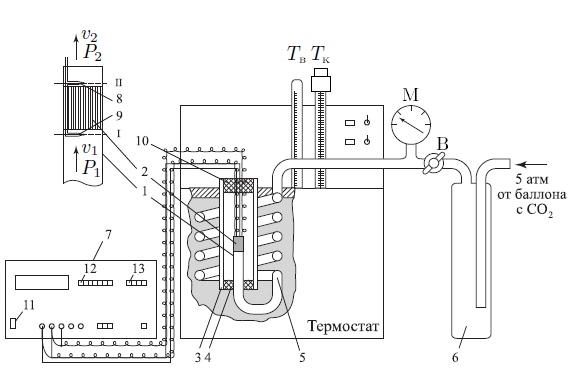
\includegraphics[scale = 0.5]{Workplace}
\end{figure}

\begin{enumerate}
\item Трубка, по которой протекает газ
\item Пористая перегородка
\item Труба Дьюара
\item Кольцо, уплотняющее трубу Дьюара
\item Змеевик
\item Балластный болон
\item Вольтметр
\item[8 и 9.] Концы термопары
\end{enumerate}

\parag {Ход работы} ~\\

\point Убедимся, что к работе можно приступать и включим термостат, выставив на нём комнатную температуру ($18^o C$).

\point Включим вольтметр в сеть, снимем его показания ($U_0$) при $\Delta P = 0$, результат запишем в табл. \ref{Tab:1}.

\point Будем повышать давление газа на $0,5$ атм., ждать установления равновесного состояния (около 5 минут) и измерять $\Delta P$ и $U$. Результаты занесём в таблицу \ref{Tab:1}.

\point С помощью формулы $\varepsilon = U(P) - U(0)$ и табл. \ref{Tab:temp} найдём $\Delta T$. Результаты внесём в табл. \ref{Tab:1}.

\begin{table}[!h]
\begin{tabular}{|c|c|c|c|c|c|}
    \hline
    Температура, $^o C$ & $0-10$ & $10-20$ & $20-30$ & $30-40$ & $40-50$ \\ \hline
    мкВ / $^o C$ & $38.8$ & $39.8$ & $40.7$ & $41.6$ & $42.5$ \\ \hline \hline
    Температура, $^o C$ & $50-60$ & $60-70$ & $70-80$ & $80-90$ & $90-100$ \\ \hline
    мкВ / $^o C$ & $43.3$ & $44.1$ & $44.9$ & $45.6$ & $46.4$ \\ \hline
\end{tabular}
\caption{Чувствительность термопары} \label{Tab:temp}
\end{table}

\begin{table}[!h]
\begin{tabular}{|c|c|c|c|c|c|c|c|c|}
    \hline
    $\Delta P$, 6 кгс/см$^2$ & $0,0$ & $8,5$ & $16,5$ & $26,0$ & $37,0$ & $41,5$ & $50,0$ & $65,0$ 
    \\ \hline
    U, мкВ & $-1$ & $-5$ & $-24$ & $-48$ & $-78$ & $-90$ & $-113$ & $-156$
    \\ \hline
    $\Delta T$, K & $0.00$ & $0.10$ & $0.58$ & $1.18$ & $1.93$ & $2.24$ & $2.81$ & $3.89$
    \\ \hline  
\end{tabular}
\caption{Результаты измерений при $T_{\text{терм}} = 18^o C$}
\label{Tab:1}
\end{table}

\point Проведём аналогичные действия для температур $T_{\text{терм}} = 30^o C$ и $T_{\text{терм}} = 50^o C$. Результаты занесём в таблицы \ref{Tab:2} и \ref{Tab:3}.

\begin{table}[!h]
\begin{tabular}{|c|c|c|c|c|c|c|c|}
    \hline
    $\Delta P$, 6 кгс/см$^2$ & $0,0$ & $9,5$ & $17,5$ & $25,5$ & $42,0
    $ & $-49,5$ & $-66,0$ 
    \\ \hline
    U, мкВ & $0$ & $-22$ & $-27$ & $-42$ & $-83$ & $-103$ & $-146$ 
    \\ \hline
    $\Delta T$, K & $0.00$ & $0.53$ & $0.65$ & $1.01$ & $2.00$ & $2.48$ & $3.51$
    \\ \hline  
\end{tabular}
\caption{Результаты измерений при $T_{\text{терм}} = 30^o C$}
\label{Tab:2}
\end{table}

\begin{table}[!h]
\begin{tabular}{|c|c|c|c|c|c|c|}
    \hline
    $\Delta P$, 6 кгс/см$^2$ & $0,0$ & $10,0$ & $16,0$ & $24,5$ & $40,5$ & $59,0$ 
    \\ \hline
    U, мкВ & $-24$ & $-26$ & $-20$ & $-36$ & $-70$ & $-113$
    \\ \hline
    $\Delta T$, K & $0.00$ & $0.05$ & $-0.09$ & $0.28$ & $1.06$ & $2.06$
    \\ \hline  
\end{tabular}
\caption{Результаты измерений при $T_{\text{терм}} = 50^o C$}
\label{Tab:3}
\end{table}

\point По таблицам \ref{Tab:1}, \ref{Tab:2} и \ref{Tab:3} построим графики $\Delta T (\Delta P)$ (т.~к. обе величены отрицательны, возьмём их по модулю для удобства).

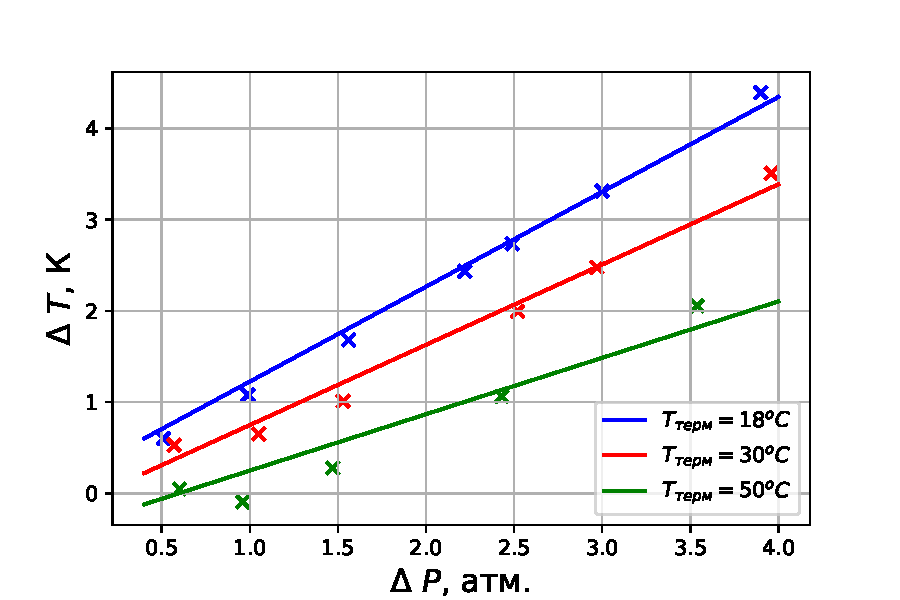
\includegraphics[scale = 0.8]{graph}

\point По графикам можно найти коэффициент Джоуля-Томсона для данных случаев как коэффициент наклона, т.~к. $\displaystyle \mu = \frac{\Delta T}{\Delta P}$

\begin{align*}
    \mu_{18} &= 1,04 ~\frac{\text{К}}{\text{атм}} = 1,03 \cdot 10^{-5} ~\frac{\text{К}}{\text{Па}} \\[3mm]
    \mu_{30} &= 0,88 ~\frac{\text{К}}{\text{атм}} = 8,68 \cdot 10^{-6} ~\frac{\text{К}}{\text{Па}} \\[3mm]
    \mu_{50} &= 0,62 ~\frac{\text{К}}{\text{атм}} = 6,12 \cdot 10^{-6} ~\frac{\text{К}}{\text{Па}} \\
\end{align*}

\point Воспользуемся выражением для $\mu$, чтобы найти коэффициенты уравнения Ван-дер-Ваальса. Для пары (1): $\mu_{18}$ и $\mu_{30}$:

\[
\begin{cases}
    \mu_{18} \cdot C_p = \dfrac{2a}{RT_{18}} - b \\[3mm]
    \mu_{30} \cdot C_p = \dfrac{2a}{RT_{30}} - b
\end{cases}
\]

Если решить систему уравнений и подставить $C_p = 40 ~\frac{\text{Дж}}{\text{K}}$, то:

\[
\begin{cases}
    a = \dfrac{R C_p (\mu_{18} - \mu_{30})}{2 (\dfrac{1}{T_{18}} - \dfrac{1}{T_{30}})} \approx 1,98 ~\frac{\text{Па м$^6$}}{\text{моль}}\\[10mm]
    b = \dfrac{C_p (\mu_{18} - \mu_{30})}{1 - \dfrac{T_{18}}{T_{30}}} - C_p \mu_{18} \approx 1,22 \cdot 10^{-3} ~\frac{\text{м}^3}{\text{моль}}
\end{cases}
\]

Аналогично для пары (2): $\mu_{30}$ -- $\mu_{50}$:

\[
\begin{cases}
    a = 2,08 ~\frac{\text{Па м$^6$}}{\text{моль}}\\[6mm]
    b = 1,31 \cdot 10^{-3} ~\frac{\text{м}^3}{\text{моль}}
\end{cases}
\]

\point Теперь можно найти температуру инверсии по формуле:
\[
T_{\text{инв}} = \frac{2a}{Rb}
\]

Для пар (1) и (2): $T_{\text{инв}1} = 390~К$, $T_{\text{инв}2} = 381~К$

\point Оценим ошибки измерений:

Из-за свойств приборов:
\[\sigma_U = 1 \text{ мкВ, } \sigma_{\Delta P} = 0,5 \text{ атм}\]

С учётом таблицы чувствительности термопары можно найти погрешность измерения разности температур:
\[\sigma_{\Delta T} \approx \frac{\sigma_U}{40 \text{ мкВ}} \approx 0.03^o C\]

Из построения прямой следует, что:
\[
    \sigma_{\mu} \approx \frac{1}{\sqrt{6}} \cdot \sqrt{\frac{\langle \Delta T^2 \rangle  - \langle \Delta T \rangle^2}{\langle \Delta P^2 \rangle  - \langle \Delta P \rangle^2} - \mu^2} \approx 4 \cdot 10^{-7} \frac{\text{К}}{\text{Па}}
\]

Следовательно:

\[\sigma_a = \frac{a}{\mu} \cdot \sigma_{\mu} \approx 8 \cdot 10^{-2} ~\frac{\text{Па м$^6$}}{\text{моль}},~ \sigma_b = \frac{b}{\mu} \cdot \sigma_{\mu} \approx 5 \cdot 10^{-5} ~\frac{\text{м}^3}{\text{моль}}\]

Тогда погрешность измерения температуры инверсии составит:

\[\sigma_{T_{\text{инв}}} = T_{\text{инв}} \cdot \sqrt{\left(\frac{\sigma_a}{a}\right)^2 + \left(\frac{\sigma_b}{b}\right)^2} \approx 30 \text{ К}\]

\parag{Заключение} Значение температуры инверсии и коэффициентов $a$ и $b$ значительно отличаются табличных:
\begin{align*}
    T_{\text{инв}} &= 2050~K \\
    a &= 0,36 ~\frac{\text{Па м}^6}{\text{моль}} \\
    b &= 43 \cdot 10^{-3} ~\frac{\text{см}^3}{\text{моль}}
\end{align*}

Следовательно, выбранная нами методика не подходила для точных измерений, а приближения, сделанные в рамках построения теоретической модели, могут оказаться неприменимыми в наших условиях.

\newpage
\parag{Черновик работы}

\begin{figure}[!h]
    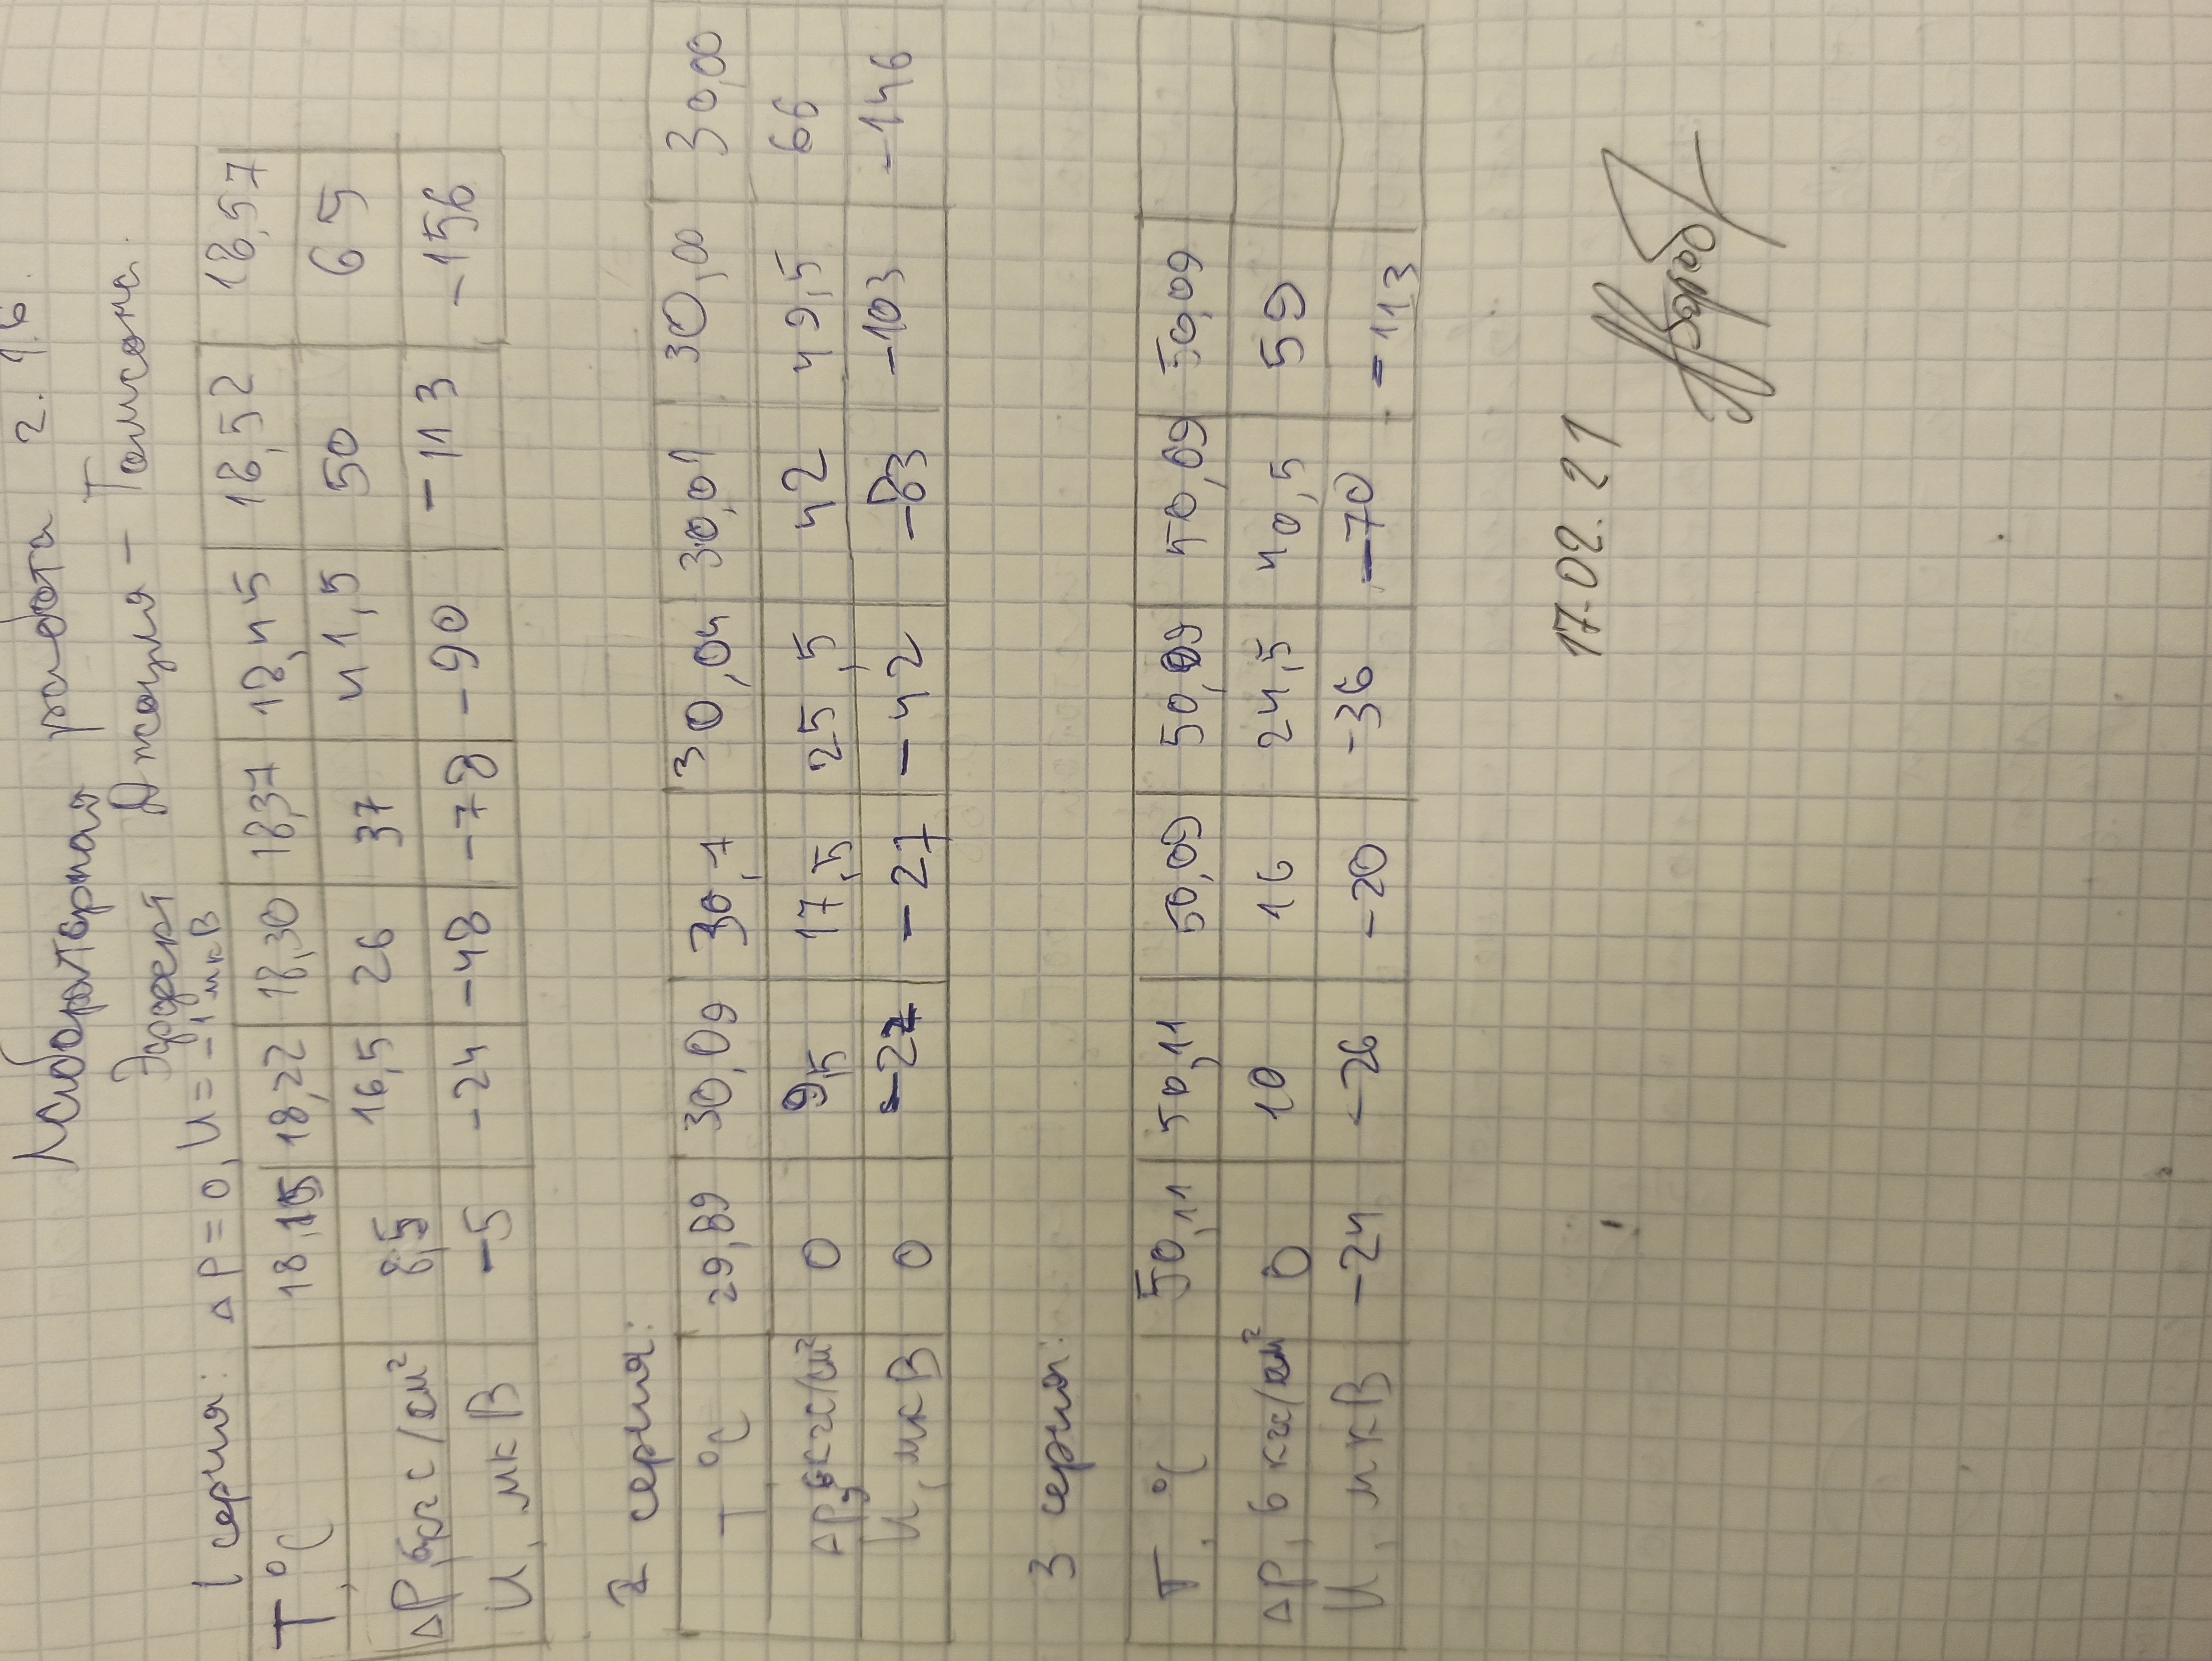
\includegraphics[scale = 0.12, angle = 270]{BlackPaper.jpg}    
\end{figure}

\end{document}
